% Copyright 2009 by Tomasz Mazur
%
% This file may be distributed and/or modified in all ways.


\documentclass[xcolor=pdftex,t,11pt]{beamer}

%%%%%%%%%%%%%%%%%%%%%%%%%%%%%%%%%%
%       SET OPTIONS BELOW        %
%%%%%%%%%%%%%%%%%%%%%%%%%%%%%%%%%%

\usepackage{xspace}
\usepackage{subfig}
\usepackage{adjustbox}
\usepackage{pifont,color,soul}
\usepackage[most]{tcolorbox}
\usepackage{listings}
\usepackage{blindtext}
\usepackage{fancyvrb}
 \usepackage{adjustbox}
\usepackage{xcolor,colortbl}
\usepackage{algorithm,algorithmic}
\usepackage{caption}
\newcommand{\xmark}{\ding{55}}
\definecolor{azure}{rgb}{0.0, 0.5, 1.0}

\lstnewenvironment{queryl}[1][] 
   {\lstset{linewidth=8cm, #1}}
   {}

\usetheme[
% Toggle showing page counter
pagecounter=true,
%
% String to be used between the current page and the
% total page count, e.g. of, /, from, etc.
pageofpages=of,
%
% Defines the shape of bullet points. Available options: circle, square
bullet=circle,
%
% Show a line below the frame title. 
titleline=true,
%
% Set the style of the title page (true for fancy, false for standard)
alternativetitlepage=true,
%
% Institution logo for fancy title page.
% Comment out to remove the logo from the title page.
% IMPORTANT: THERE IS A BUG IN SOME VERSIONS OF PDFLATEX AND FONTS
% ON THE LOGOS ARE NOT RENDERED PROPERLY. IN SUCH A CASE ADD `2` 
% TO THE NAME OF THE LOGO, E.G. comlab2 INSTEAD OF comlab
%titlepagelogo=images/titlepage/ou,
%
% Department footer logo for fancy title page
% Comment out to remove the logo from the footer of the title page/
% IMPORTANT: THERE IS A BUG IN SOME VERSIONS OF PDFLATEX AND FONTS
% ON THE LOGOS ARE NOT RENDERED PROPERLY. IN SUCH A CASE ADD `2` 
% TO THE NAME OF THE LOGO, E.G. comlab2 INSTEAD OF comlab
%titlepagefooterlogo=images/titlepage/comlab,
%
% Institution/department logo for ordinary slides
% Comment this line out to remove the logo from all the pages.
% Available logos are: ou, comlab, comlabinline, comlabou
% IMPORTANT: THERE IS A BUG IN SOME VERSIONS OF PDFLATEX AND FONTS
% ON THE LOGOS ARE NOT RENDERED PROPERLY. IN SUCH A CASE ADD `2` 
% TO THE NAME OF THE LOGO, E.G. comlab2 INSTEAD OF comlab
%ordinarypageslogo=TU-Signet,
%
%
% Add watermark in the bottom right corner
%watermark=<filename>,
%
% Set the height of the watermark.
%watermarkheight=100pt,
%
% The watermark image is 4 times bigger than watermarkheight.
%watermarkheightmult=4,
]{Torino}

% Select color theme. Available options are:
% mininmal, greenandblue, blue, red
\usecolortheme{blue}

%Select different font themes.Available options are:
% default, serif, structurebold, structureitalicserif, structuresmallcapsserif
\usefonttheme{structurebold}


\pgfdeclareimage[height=6ex]{ou-logo}{ou}

\logo{\pgfuseimage{ou-logo}}

\usepackage{pgf}

\pgfdeclareimage[height=6ex]{ou-logo}{ou}

\logo{\pgfuseimage{ou-logo}}

\usepackage{listings}

%% \lstset{language=C,
%%   basicstyle=\normalsize,
%%   linewidth=8cm
%%  }

\usepackage{ifthen}

\usepackage{pgf}
\usepackage{tikz}
\usetikzlibrary{arrows, automata, shapes.multipart, chains, positioning, fit, graphs, spy, shapes, backgrounds, patterns}

\usepackage{color}
\definecolor{light-gray}{gray}{0.80}
\definecolor{green}{rgb}{0.30588, 0.60392, 0.023529}     % #4e9a06


\newenvironment<>{codeblock}[1][]{%
  \setbeamercolor{block title example}{fg=white,bg=blue!75!black}%
  \begin{block}#2[#1]}{\end{block}}

  \newenvironment<>{examplesecond}[1]{%
  \setbeamercolor{block title}{fg=white,bg=blue!75!black}%
  \begin{block}#2{#1}}{\end{block}}

  

%%%%%%%%%%%%%%%%%%%%%%%%%%%%%%%%%%
%       PRESENTATION INFO        %
%%%%%%%%%%%%%%%%%%%%%%%%%%%%%%%%%%

  \title{\fontsize{11}{12}\selectfont DSSynth: An Automated Digital Controller Synthesis Tool
    \newline
     for Physical Plants.}
\subtitle{ASE 2017}
\institute{\normalsize Diffblue Ltd., \\University ~of ~Oxford, \\Federal University of Amazonas}
\date{November, 2017.}
\author{\normalsize Alessandro Abate, Iury Bessa, Dario Cattaruzza,\\
  Lennon Chaves, Lucas Cordeiro, Cristina David,\\
  Pascal Kesseli, Daniel Kroening and Elizabeth Polgreen}

\begin{document}


%%%%%%%%%%%%%%%%%%%%%%%%%%%%%%%%%%
%       SLIDE DEFINITIONS        %
%%%%%%%%%%%%%%%%%%%%%%%%%%%%%%%%%%

\begin{frame}[plain]
  \titlepage
  \vspace{-3.5cm}
   % 
\includegraphics[width=.15\textwidth]{figures/aec-badge-cav.pdf}
\end{frame}


\begin{frame}{Motivation}

\centering
 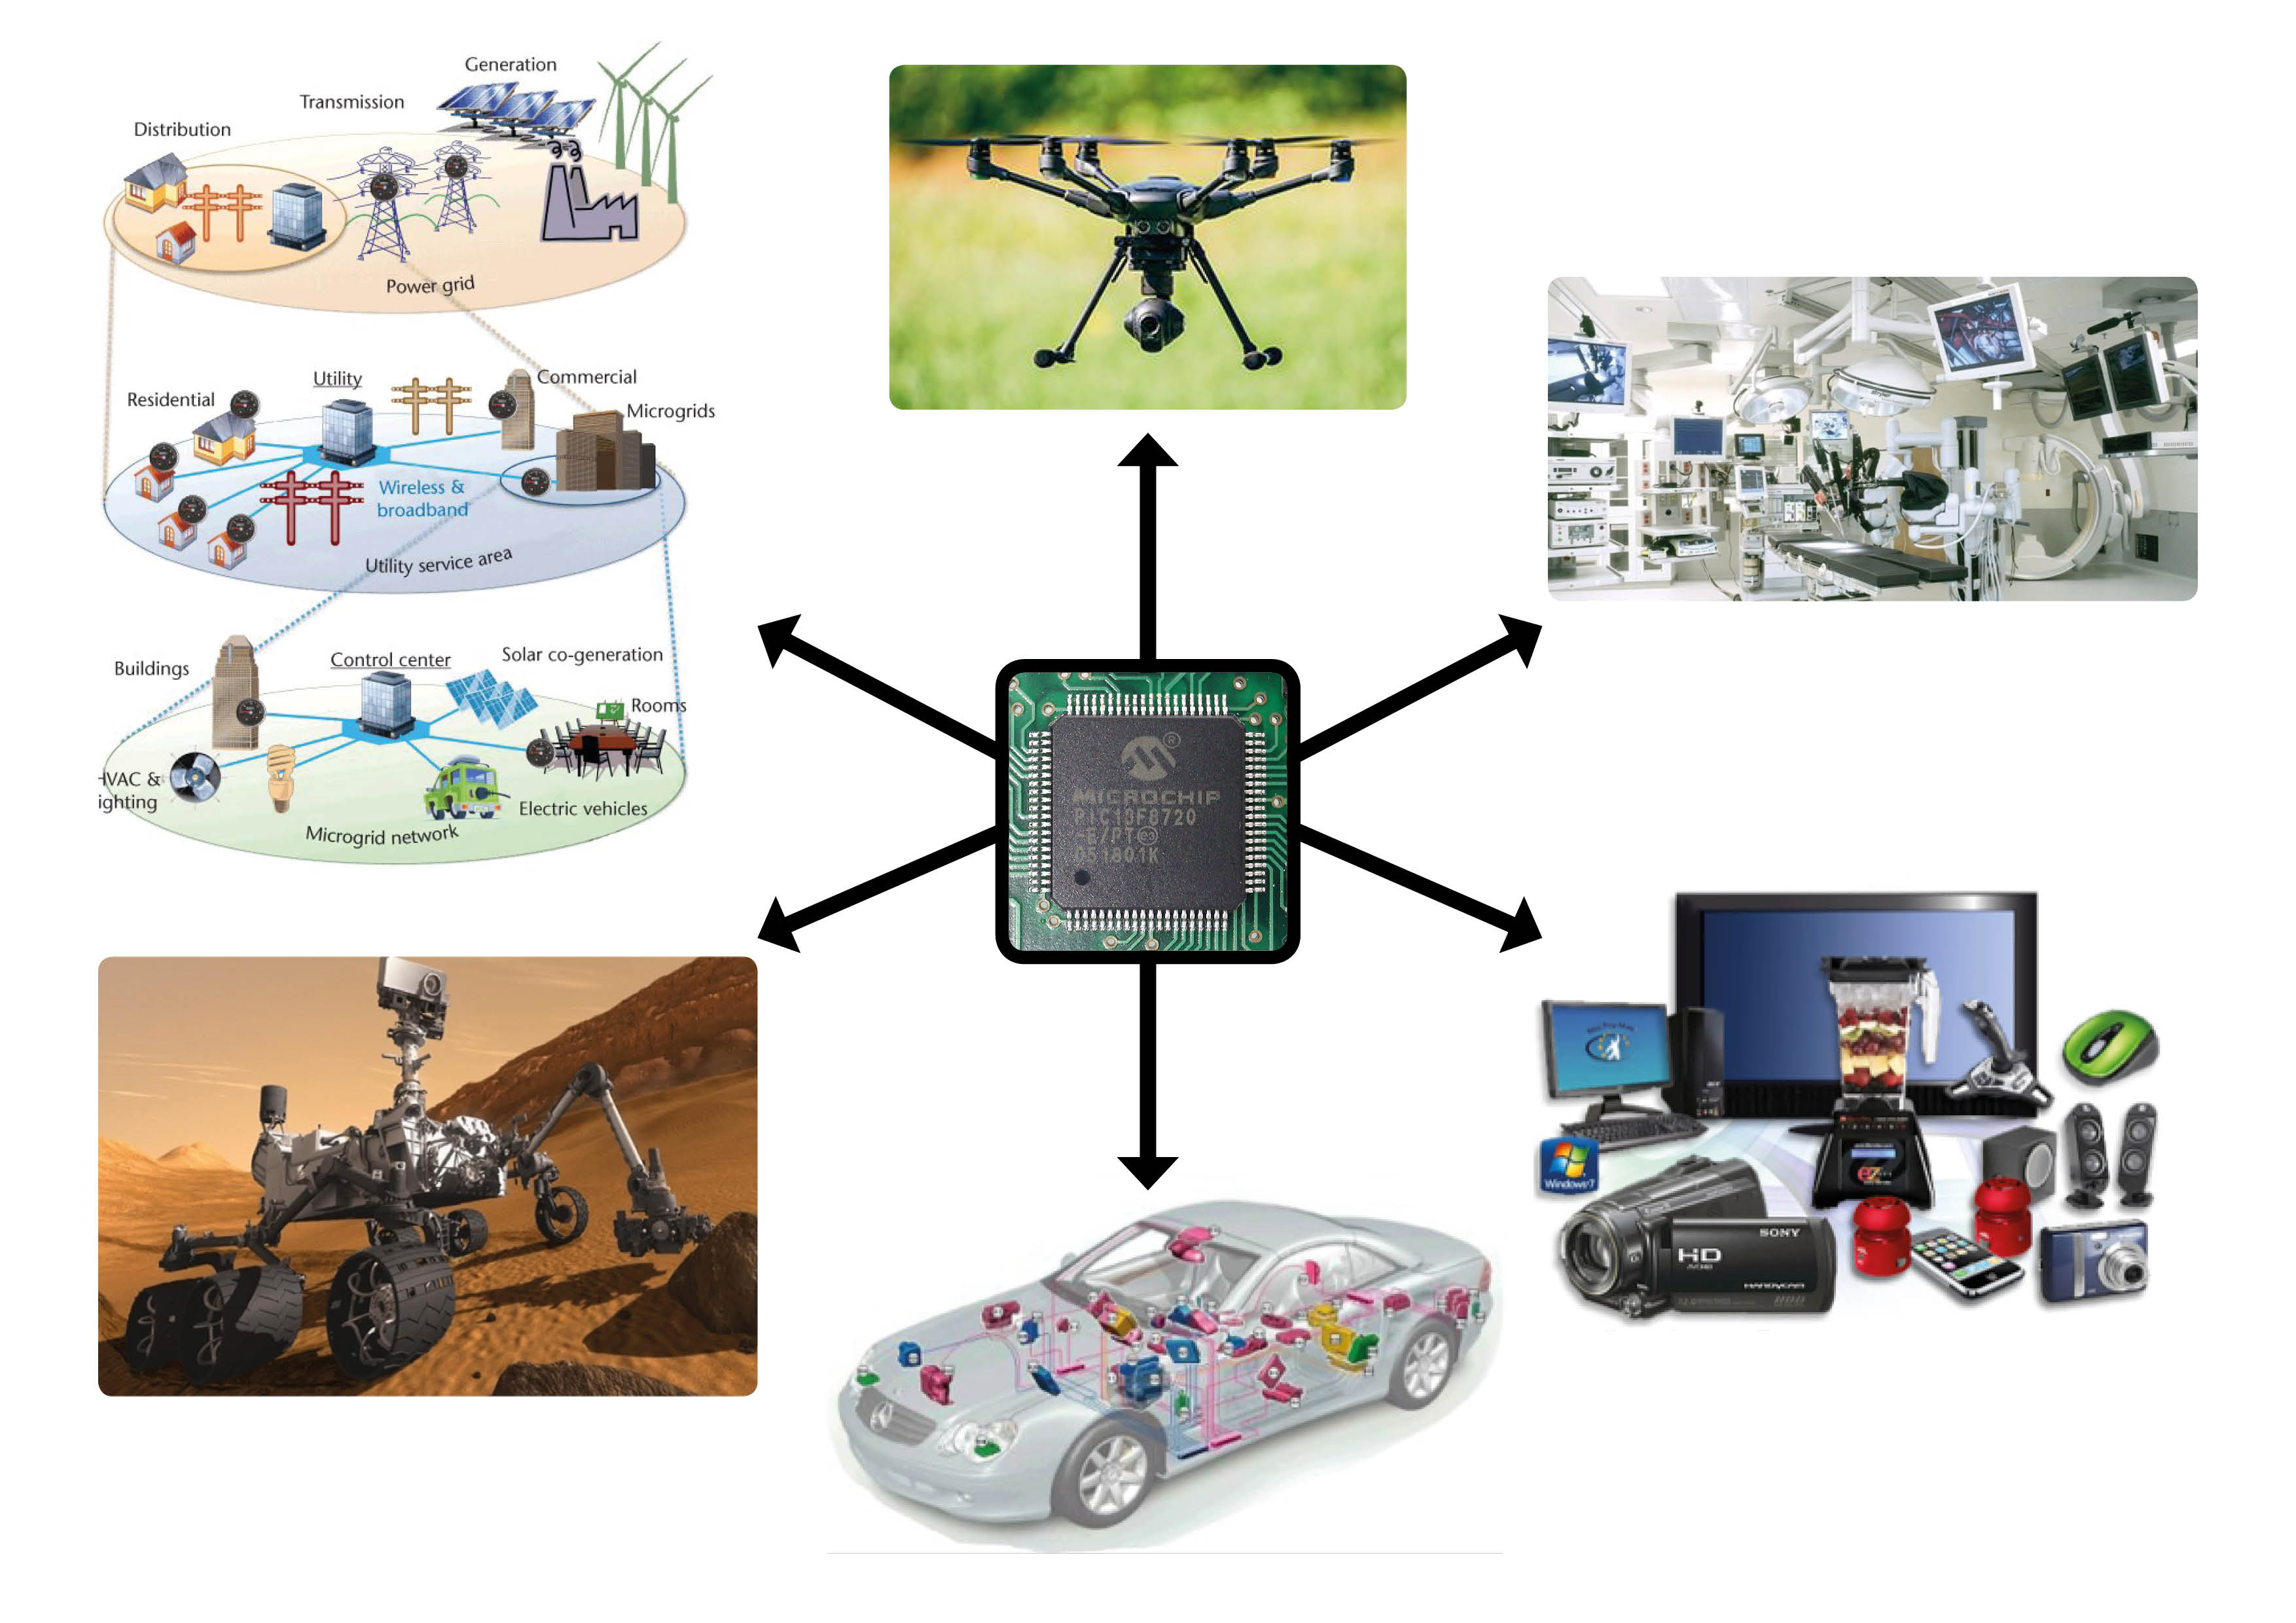
\includegraphics[width=.75\textwidth]{figures/controller.jpg} 

 
\uncover<2>{
 %\vspace{-.5cm}
  \small
{\bf Automatically synthesise feedback digital controllers that ensure
{\color {red} stability} and {\color {red} safety}}}

\end{frame}

\begin{frame}{State-feedback architecture}
\vspace{-1cm}
\begin{center}
  \begin{overprint}
    \onslide<1,2>
    \centerline{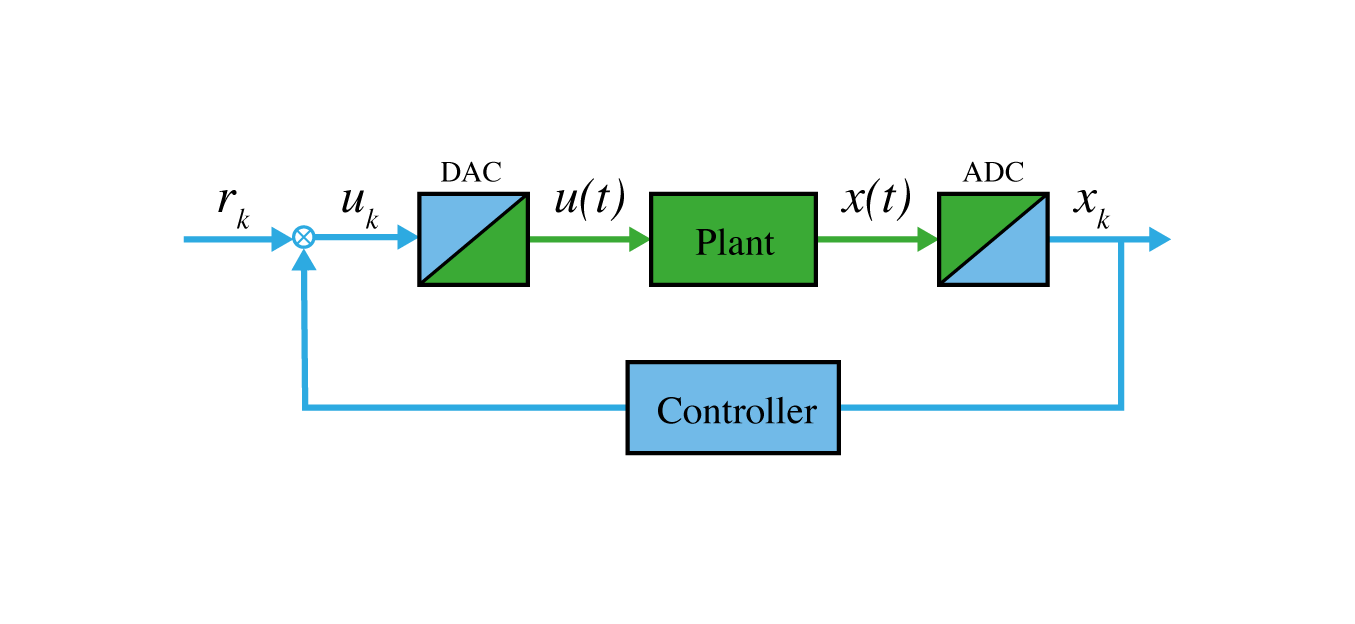
\includegraphics[width=.9\textwidth]{figures/spirals/diagram-15.png}}
    %% \onslide<3->
    %% \centerline{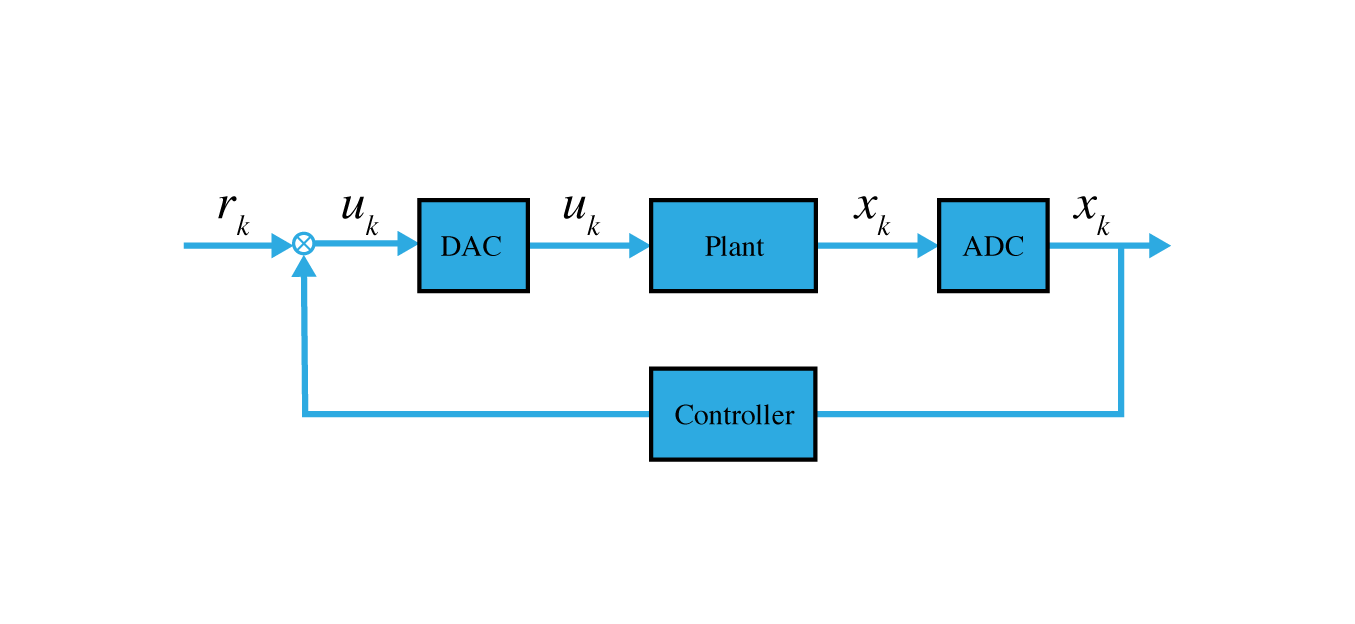
\includegraphics[width=.9\textwidth]{figures/spirals/diagram-16.png}}
  \end{overprint}
  \end{center}
  \vspace{-1cm}
  \only<1,2>{{\bf Continuous-discrete system}}
  %\only<3->{{\bf Digital domain}}  
  \begin{itemize}
  \item \only<1,2>{\colorbox{green!70}{Plant:
    \textsc{$\dot{x}(t) = Ax(t)+ Bu(t), \quad t \in \mathbb R_0^+,~x(0)=initial~state$}}}
    %% \only<3->{\colorbox{azure!70}{Plant:
    %% \textsc{$x_{k+1} = A x_k+ B u_k, \quad k \in \mathbb \mathbb N,~x_0=initial~state$}}}
  \item \colorbox{azure!50}{State-feedback controller:   \only<1>{$u_k = r_{k} - C x_k$}\only<2->{$u_k = - C x_k$}}
  %\item \uncover<4->{Finite precision}  
\end{itemize}
\end{frame}

\end{document}
